\subsection{Other Metrics}\label{append:other metrics}

We also evaluate correlations between accuracy and the following metrics:
\begin{itemize}
    \item \texttt{Review Centroid}: the median position of all \review\ chunks within a trace, normalized to $[0,1]$.
    \item \texttt{Review Chunk Fraction}: the fraction of chunks labeled \review\ among all chunks.
    \item \texttt{Review$\rightarrow$Progress Switch Count}: the number of transitions where a \review\ chunk is followed by a \progress\ chunk, normalized by the total number of chunks.
    \item \texttt{Motivation Score}: the fraction of \review\ chunks that state a clear motivation for the action (details in Appendix~\ref{append-motivation}).
    \item \texttt{First Failed-Step Depth}: the depth of the first failed step in the reasoning graph.
    \item \texttt{Reasoning Depth}: the depth of the reasoning graph from the problem statement.
\end{itemize}

\paragraph{Results.}
Figure~\ref{fig:motivation_all_correlation} reports the correlations. Many effects are not consistent across models, for example, the position of \Review\ often behaves like a model-specific stylistic feature rather than a general predictor. Nonetheless, we observe the following patterns:
(i) Correlations are stronger and more frequent in math reasoning than in general scientific reasoning;
(ii) \texttt{Review-Chunk Fraction} shows weaker and more unstable association with accuracy, compared with \fsf, suggesting that graph-level metrics are the more informative granularity;
(iii) \texttt{Motivation Score} exhibits mixed, model-dependent correlations. This feature is intuitively important for human reasoning, as it gauges whether each action is taken with a clear purpose. For LRMs, however, it shows no consistent correlation with accuracy, suggesting their reasoning dynamics can differ from human patterns. (iv) For math reasoning, nearly all models show a positive association between \texttt{Reasoning Depth} and accuracy.

In addition to these metrics, we report analyses of other graph-based measures as well as entropy and progressiveness; see Appendices~\ref{appendix:graph} and \ref{append:further}. A model-level correlation analysis in Appendix~\ref{append:further} shows that models exhibit different generation styles, so comparing metrics \emph{across} models may be biased. This supports our methodology: estimate correlations \emph{within} each model, then seek patterns that replicate \emph{across} models.



% \todo{Create a distributional graph for length, review ratio, for math and GPQA}

% \todo{plot the distribution of failed steps across different models. Do better model good at having more backtracking?}

% \todo{We could also talk about how different model differ in these metrics; Does model A has more accuracy by having metric B higher than Model C?}

\begin{figure}[tb]
    \centering
    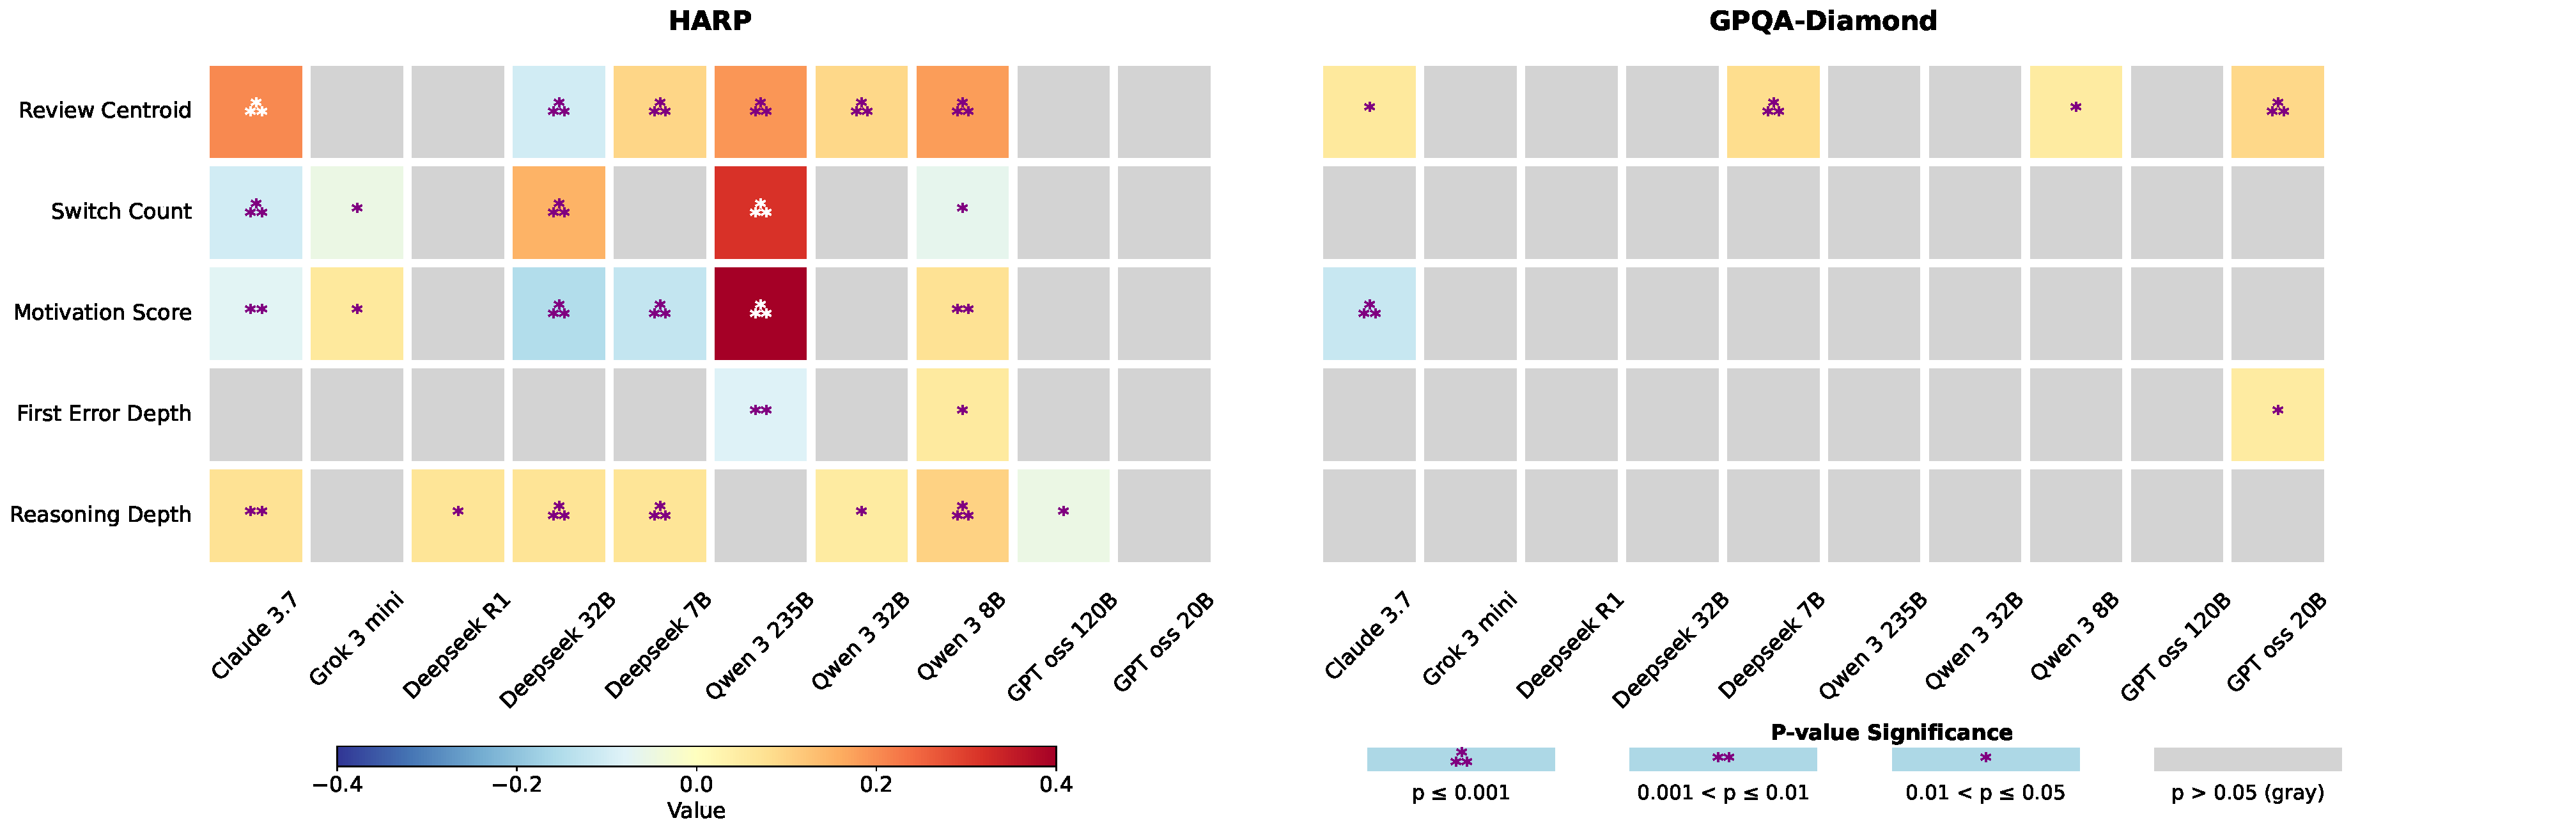
\includegraphics[width=1.08\linewidth]{final_figs/correlation_motivation.pdf}
    \caption{Conditional correlations computed on the full dataset, for \Review position, \texttt{Motivation Score}, \texttt{First Failed-Step Depth}, and overall \texttt{Reasoning Depth}. Again, correlations are shown with a color scale; non-significant cells (\(p>0.05\)) are grayed out, and * denotes statistical significance (see the legend). We color * white or purple for visualization only. }
    \label{fig:motivation_all_correlation}
\end{figure}